Organizing the \gdomeditor{} into categories (\bxfigref{OMCats}) makes it easier to find components you have mapped later on -- especially if you have to remap any of them. As a general rule, the categories in the \gdomeditor{} will reflect the categories in the \gdtestcasebrowser{} in the \bxname{\gdaut{}-bound modules} category -- the \gdaut{} should be split up into areas and dialogs, so that you have a simple yet hierarchical overview of your \gdaut{} in the \gdomeditor{} \bxpref{BPCategories}. 

\begin{figure}[h]
\begin{center}
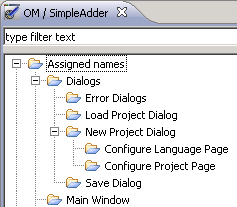
\includegraphics{BestPractices/Structure/PS/OMCats}
\caption{Categories in the \gdomeditor{}}
\label{OMCats}
\end{center}
\end{figure} 
